\section{Brugerflade}
\textit{For at børnene kan blive aktiveret, er det væsentligt at have en brugerflade, som motiverer dem.}
\subsection{Design}
Brugerfladen benyttes til at motivere børn til en mere aktiv hverdag. Dette gøres ud fra \secref{motivation_boern}, hvor det beskrives at børn motiveres gennem succesoplevelser. Brugerfladen designes dermed ud fra at alle børn har mulighed for at opnå mange point, da pointene vægtes ud fra intensiteten af en given aktivitet og ikke blot aktivitetstypen.

Data fra algoritmen sendes til matlab, som det ses på \figref{fig:GUI}. Fra accelerometeret sendes data som en værdi for maxpeak, og som tiden der er gået mellem to peaks relateret til henholdsvis gang og løb. For pulssensoren sendes data som pulsen, og for gyroskopen sendes tiden der er cyklet \fxnote{Undersøg cykel}. 
Der er bestemt et threshold for gang og løb, hvormed maks-peaks mellem 100 og 1100 betegnes som gang og maks-peaks over 1100 betegnes som løb. Tiden for de registrerede maks-peaks ligges over i en tidsvariabel for den tilhørende aktivitet. Denne vises som værdi for den enekelte aktivitet, så barnet og forældrene kan se hvor længe barnet har været aktiv ved de enkelte aktiviteter. \newline
Hver aktivitet belønnes forskelligt, da det er mere væsentligt at få børnene ti lat løbe og cykle end at gå. Dermed ganges tiden for løb med en faktor 3, cykling med en faktor 2 og gang med en faktor 1. Derudover belønnes barnet for intensiteten af aktiviteten, hvormed de yderligere får dobbelt så mange point for aktiviteter med høj intensitet og 50\% mere for aktiviteter med moderat intensitet. Pointene vises ud for den enkelte aktivitet, så barnet kan se hvor mange point de har opnået ved udførslen for den enkelte aktivitet.\newline
For at aktivere børnene hver dag, samles dagens point for alle aktiviteter udført i løbet af dagen. Pointene vises grafisk som en søjle hvormed barnet nemt kan få et overblik over point fra de forskellige dage.

\begin{figure}[H]
	\centering
	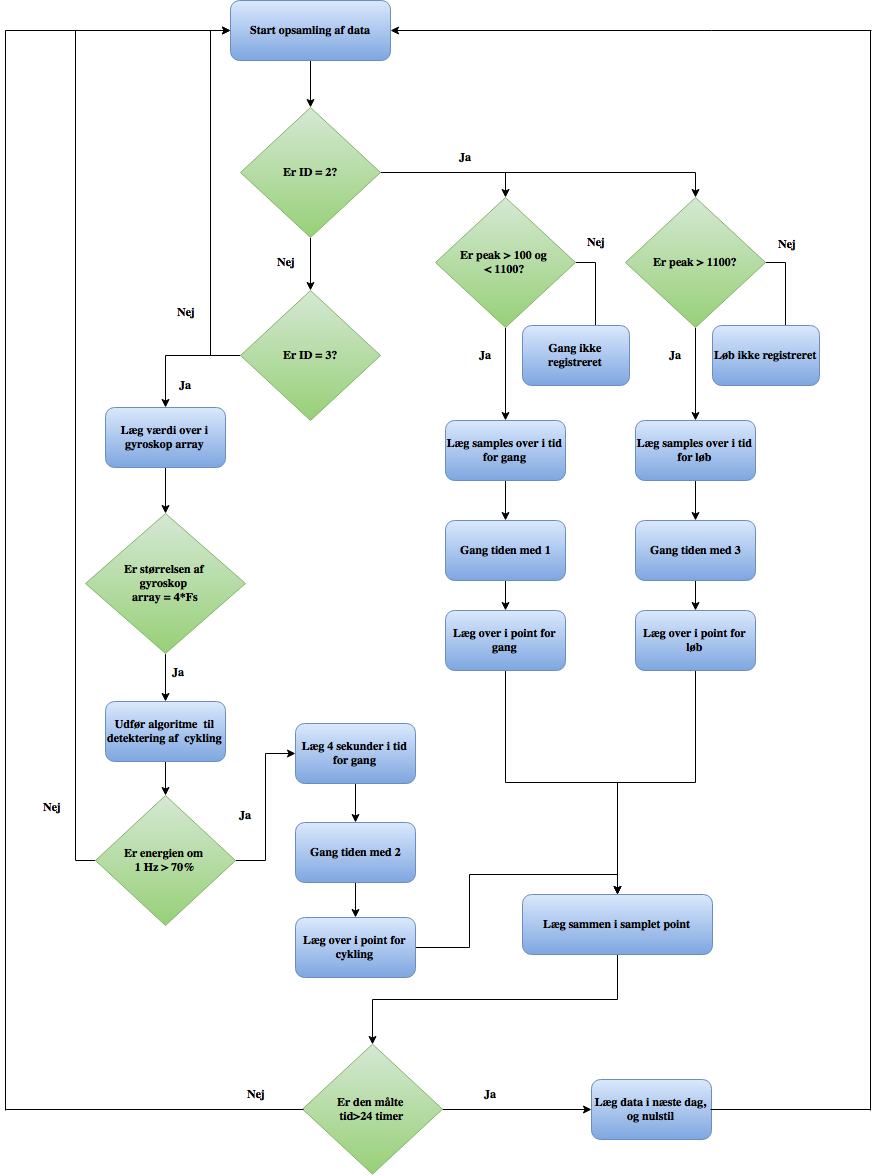
\includegraphics[scale=0.4]{figures/cDesign/pseudo_GUI.png}
	\caption{På figuren ses et flowchart som gennemgår den måde aktiviteterne behandles efter de har været gennem algoritmen.}
	\label{fig:GUI}
\end{figure}

\subsection{Implementering}
Til implementeringen anvendes matlabfunktionen Graphical User Interface (GUI), som er en funktion der gør det muligt at lave en specifik brugerflade. I GUIen benyttes en toggle button for at starte og slutte indsamling af data fra accelerometeret, gyroskopet samt pulssensoren. Derudover benyttes axes, som skal repræsentere de samlede point der er samlet i løbet af dagen. Sidst benyttes static text til de resterende bokse. \newline
Signalerne fra LSM9DS1 og pulssensoren hentes ind til matlab, hvor de ligger i en variabel med (samples, maks-peak)\fxnote{find ud af hvordan puls kommer ind}.